%---------------------------------------------------------------------
% !TEX root = 5Blman.tex
%---------------------------------------------------------------------

\chapter{Electric Fields and Potentials}

\begin{multicols}{2}
\section{Purpose}
The purpose of this laboratory exercise is to map lines of equipotential (constant voltage) and, from those lines, to determine the associated electric field lines. This hands-on experience will help you to understand concepts of potential (voltage) and its relationship with electric forces and fields.  These concepts are also explored in lecture, your text, and in homework questions and problems.
\section{Preparation}
Read or reread the appropriate sections in your text before coming to lab. Pay special attention to basic definition of electric potential the relation between equipotential lines and electric field lines, especially the way these are drawn in diagrams. The electric field and potential are related by the expression

\begin{equation} \label{e:EandV} E  = \frac{\Delta V}{\Delta d} \end{equation}

\noindent where $\Delta d$ is the distance between any two equipotential lines.

%\paragraph{Short quiz} Be prepared to take a short quiz at the beginning of lab related to the activities and the concepts of equipotential (constant voltage) lines and electric field lines.

\section{General Information}

This laboratory exercise actually simulates electrostatic fields produced by static charge distributions.  The situations discussed in the text and in class are for static distributions of charge.  It turns out to be extremely difficult to measure potentials (voltages) in truly static situations.  For example, if you apply a constant voltage between two plates and measure the voltages in between them in a tray of water, $+$ and $-$ ions actually move through the water.  Moreover, electrolysis and layers of ions at surfaces can and will distort the fields.  Measurement difficulties are overcome by using AC (alternating current), as we do in this exercise.  Best of all, the results are identical to what would be obtained in a static situation if the measurement difficulties for such static situations could be overcome.

\section{Electric field lines and potentials}
The diagram in \reffig{f:fig1} shows the basic set up.  A transformer with a nominal output of 6.3 VAC is connected to two metal bars in a clear tray partially filled with water.  An AC voltmeter is used to measure voltages surrounding the bars (which simulate parallel metal plates with a static voltage or potential between them).  The common ($-$) terminal of the AC voltage supply and the AC voltmeter are connected to the same plate.  A probe with a pointed metal tip is inserted into the water to measure voltages and to mark the plastic sheet at the bottom of the tray.  The general idea is to measure a voltage at some location and look for other locations that have the same voltage.  Doing so, you map out a number of equipotential lines parallel to the metal surface. The electric field lines will be perpendicular to the potential lines.

\begin{center}
%\begin{figure}
%	\centering
	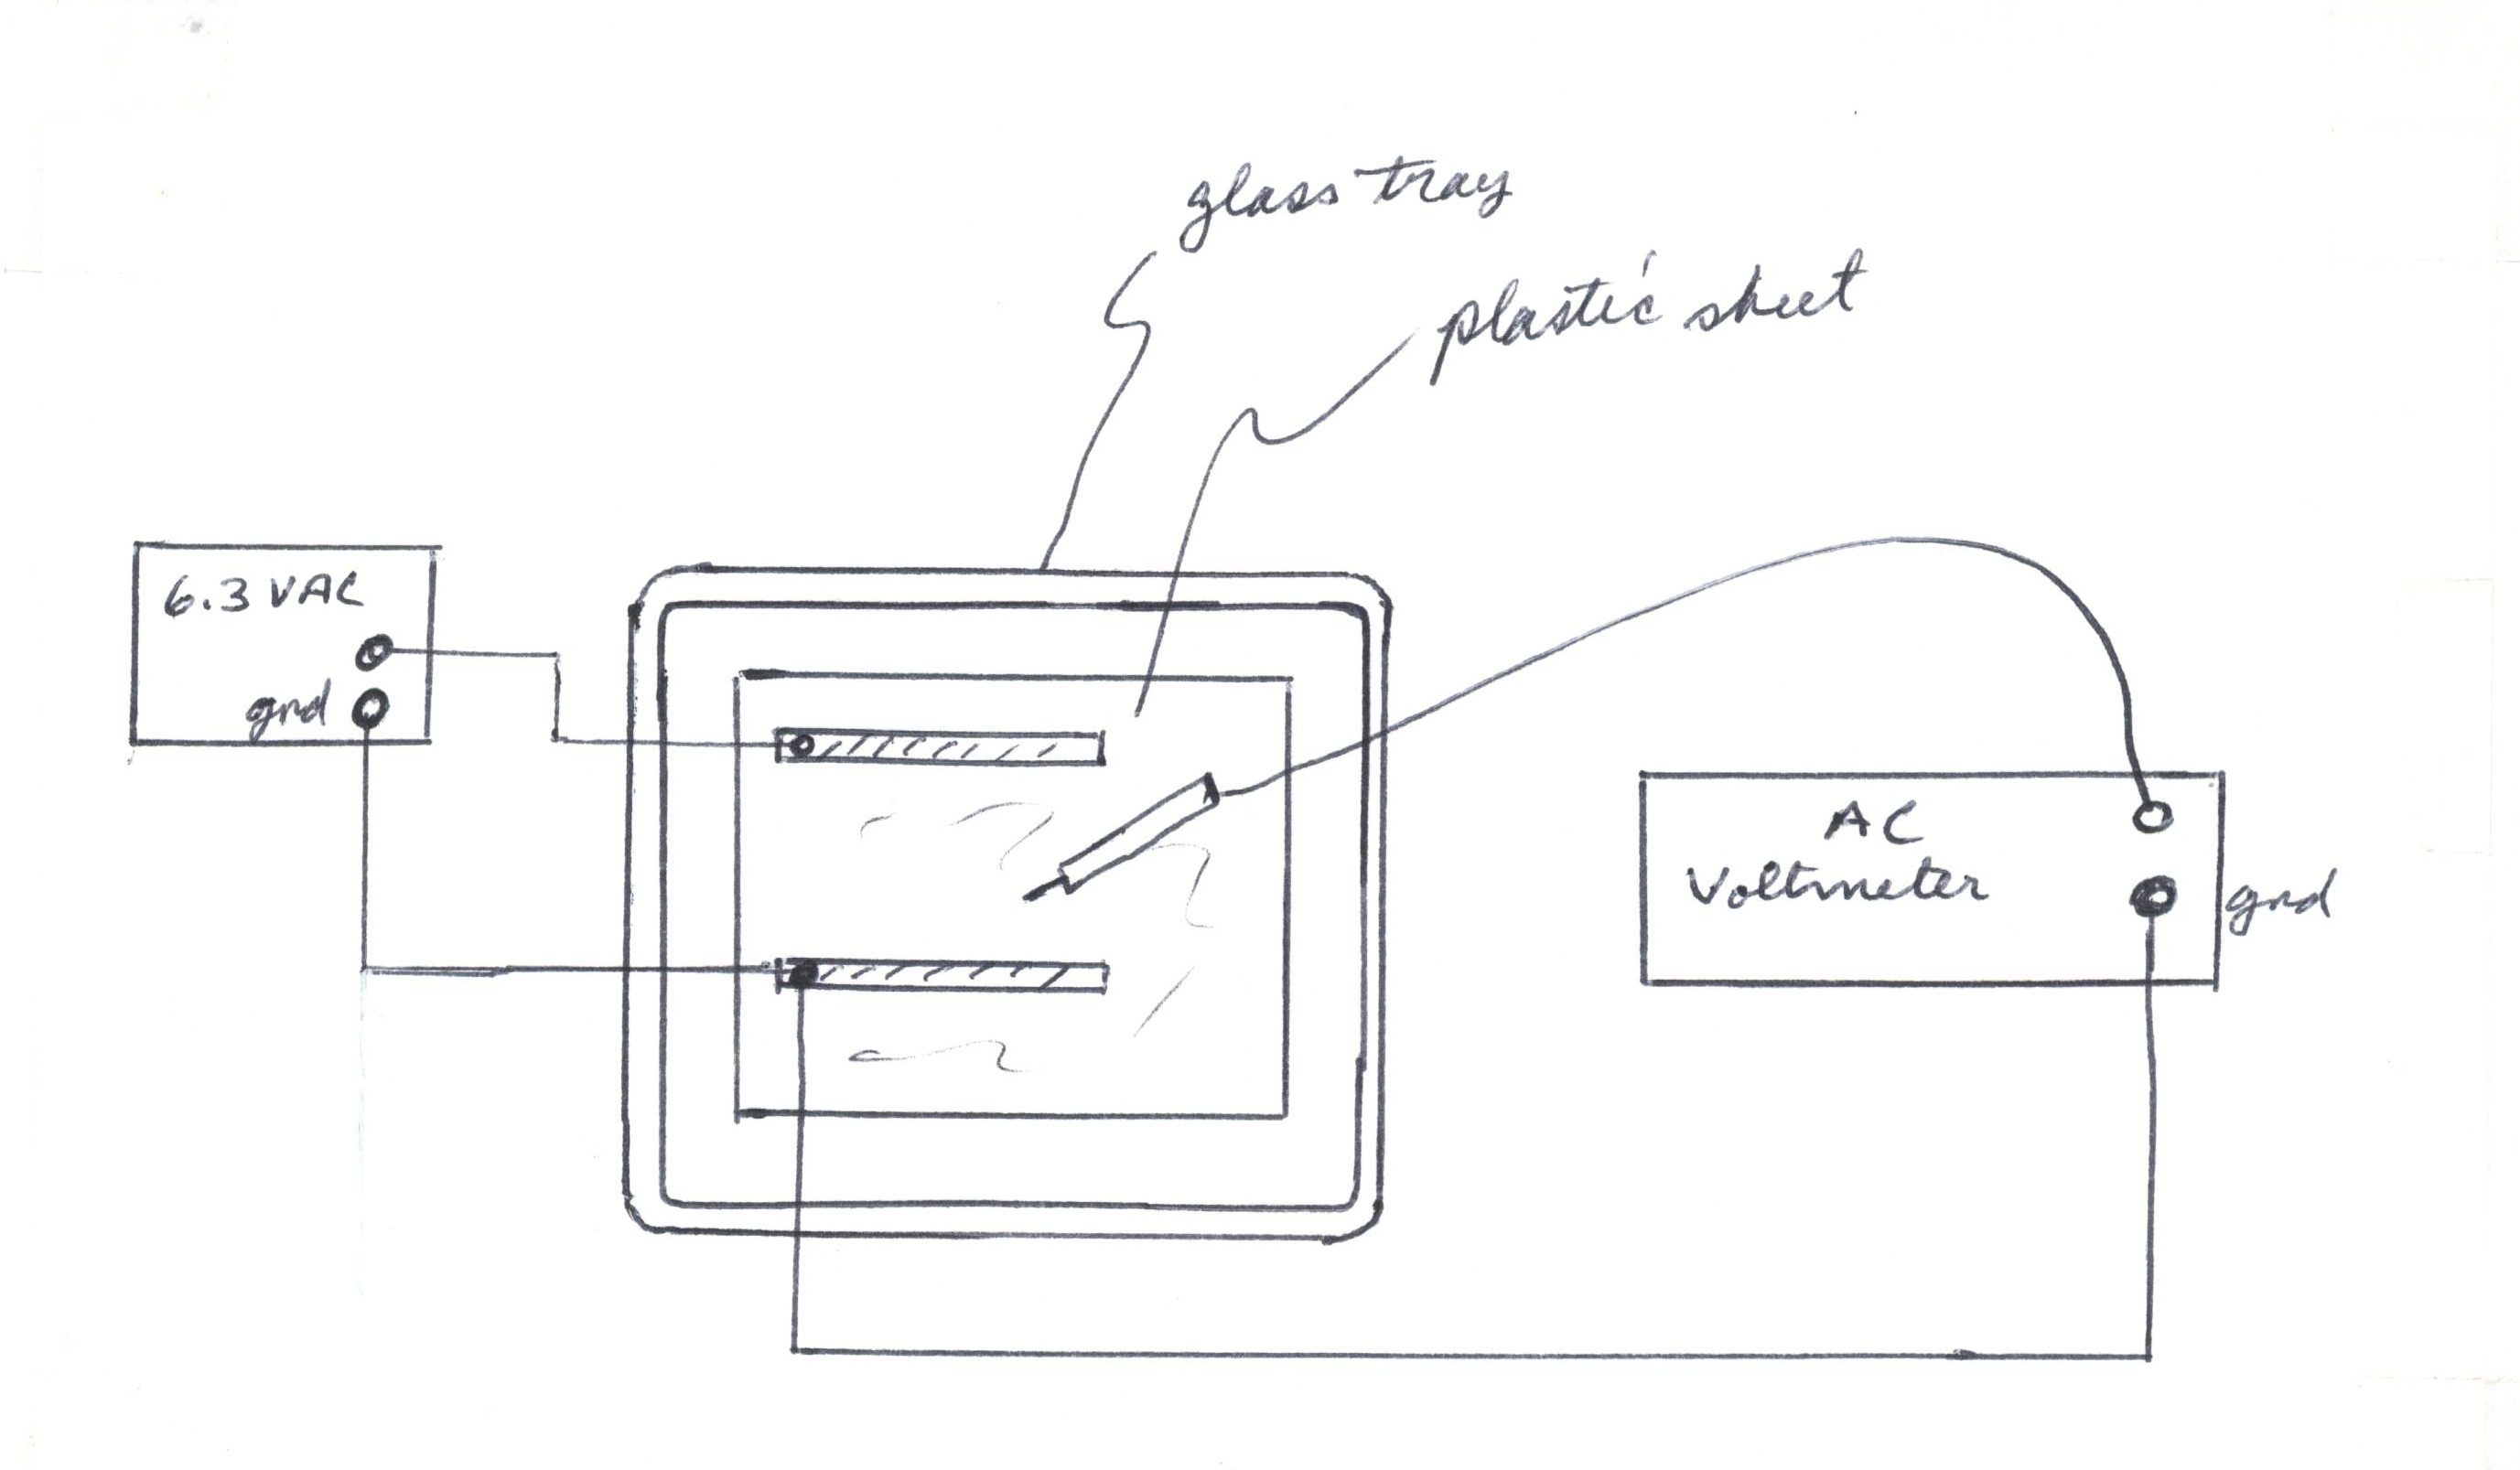
\includegraphics[scale=0.5]{5bgraf/fig_1}
%	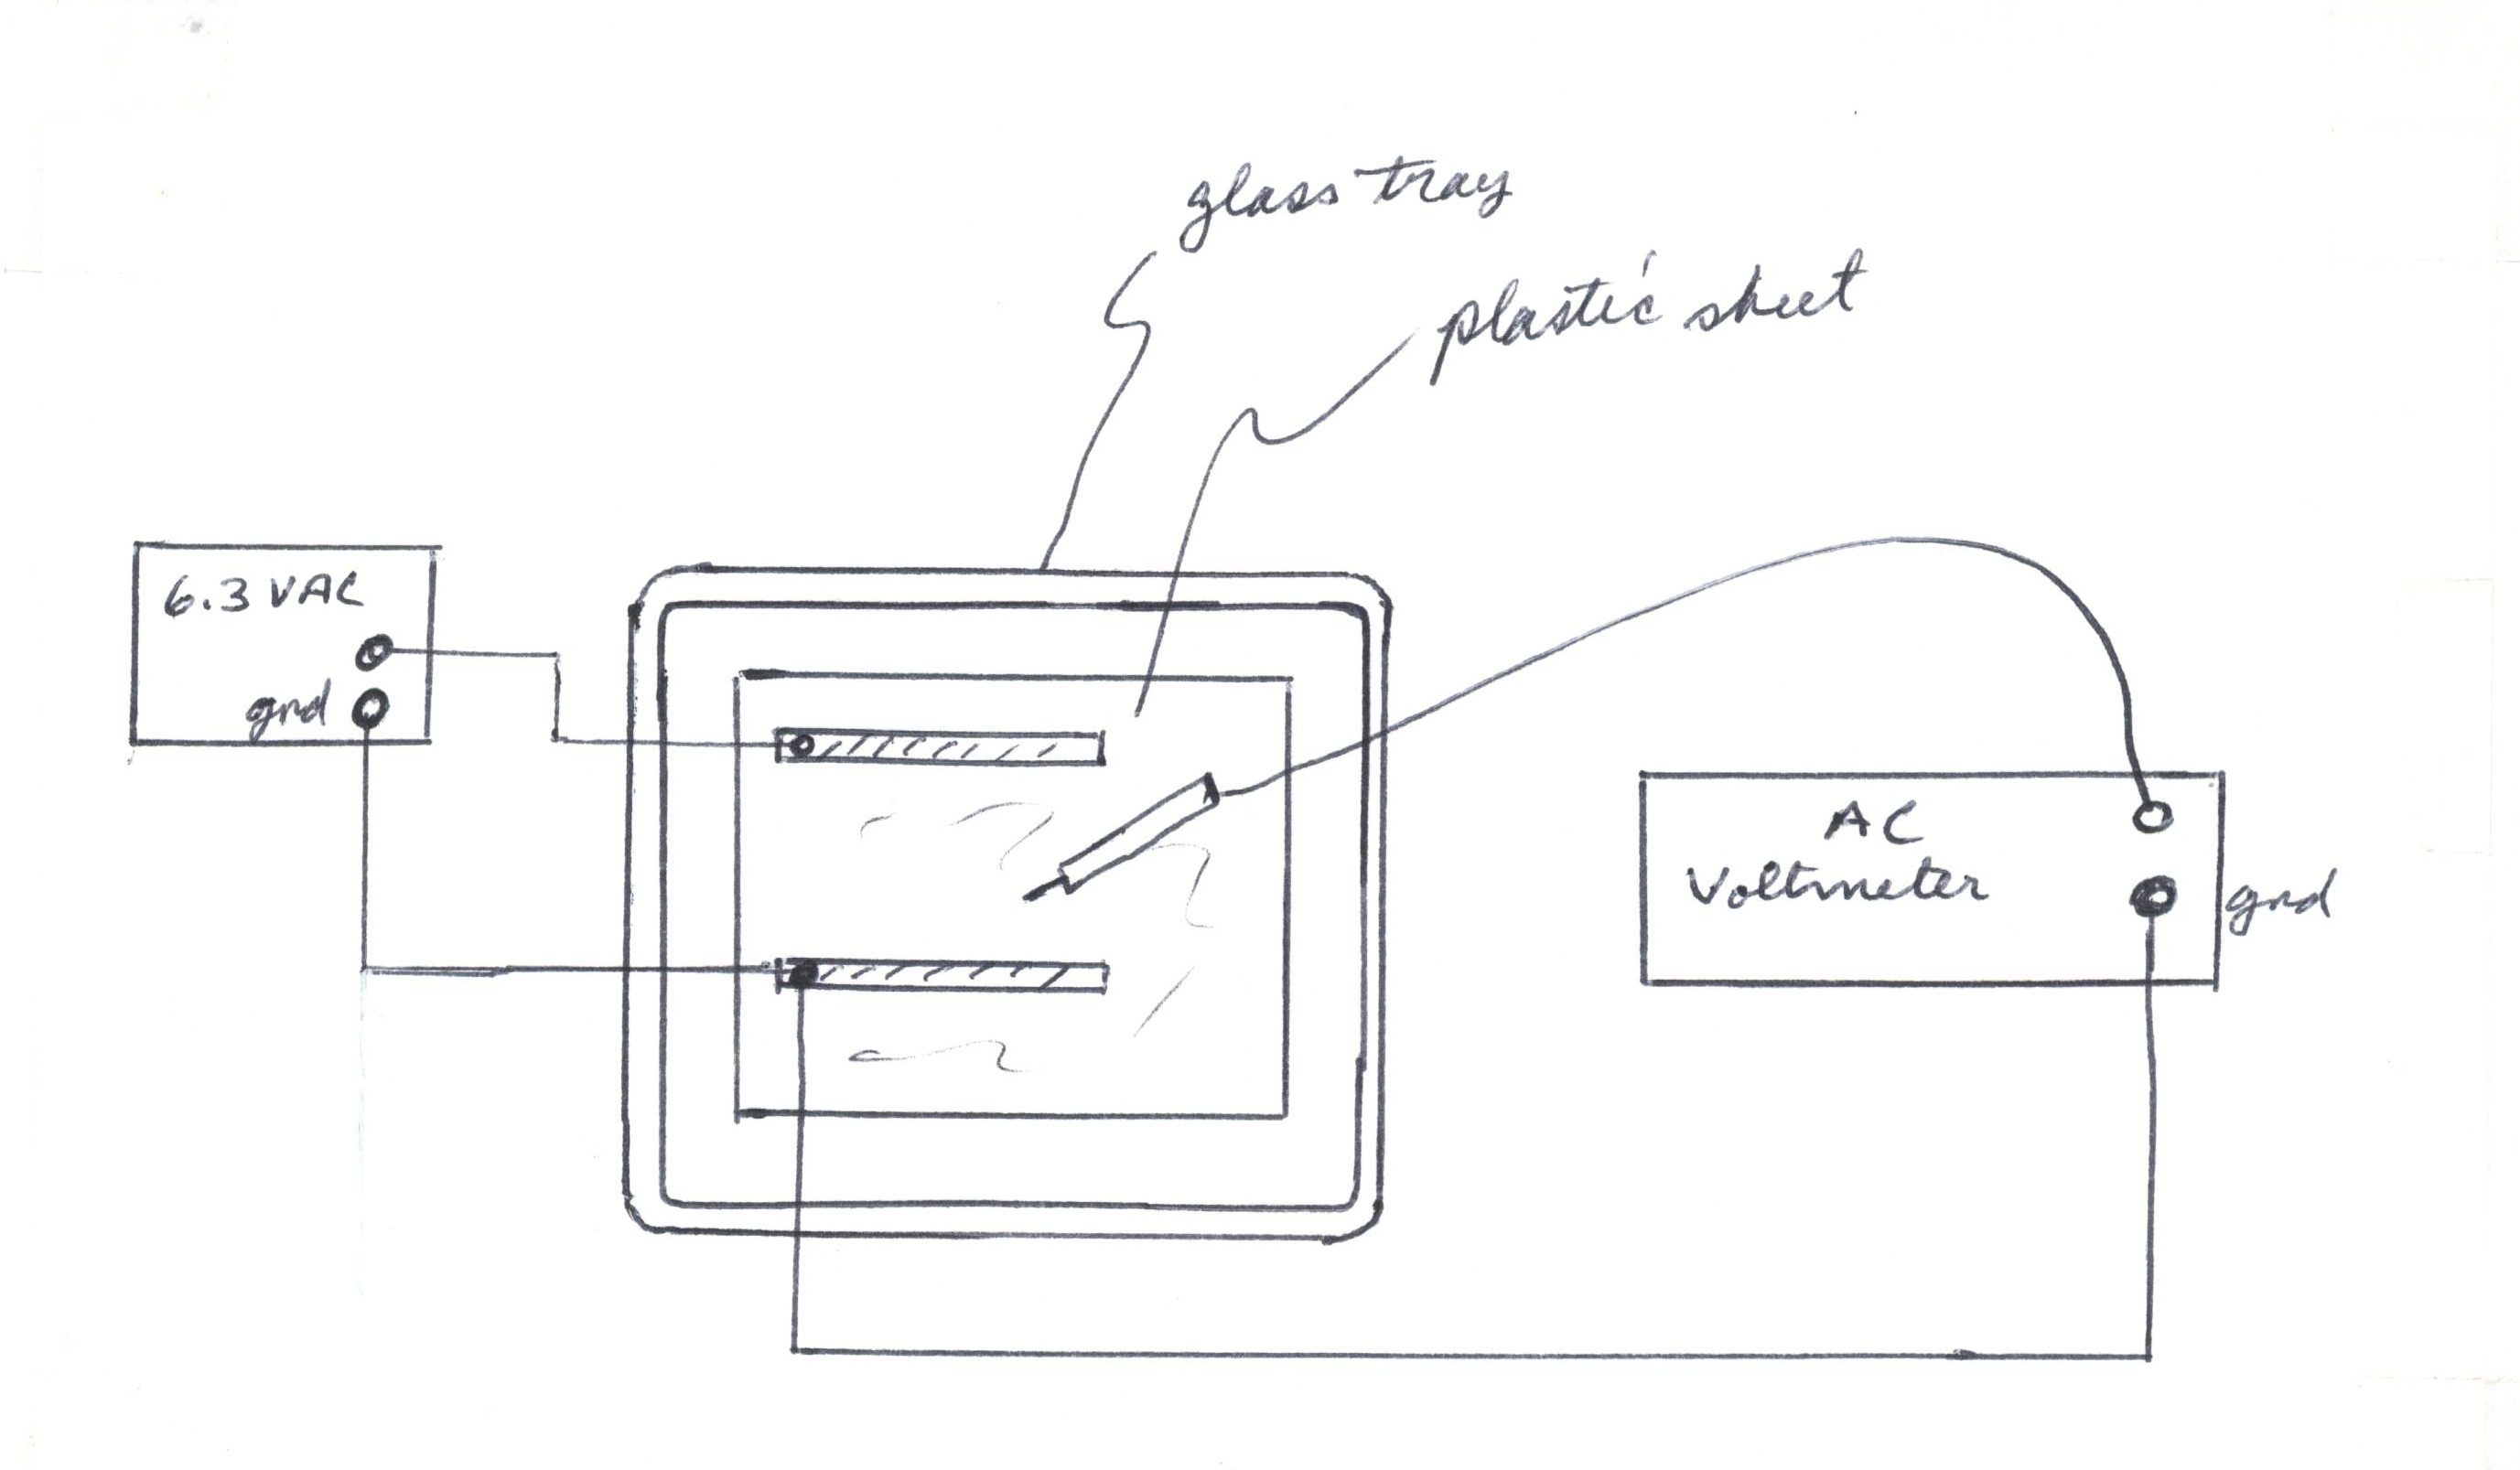
\includegraphics[bb = 20 0 400 200]{5bgraf/fig_1}
%	\caption{This simulation of charged plates allows you to map the electric potentials and determine the electric field between the plates.}
	\mfcaption{This simulation of charged plates allows you to map the electric potentials and determine the electric field between the plates.}
	\label{f:fig1}
%\end{figure}
\end{center}

\subsection{Activity: Parallel plates} %\label{s:plates}
\begin{enumerate}
	 \item Set up the two parallel bars as shown in \reffig{f:fig1} to simulate the potentials and fields surrounding parallel plates.
	 \item  Take data on a clear plastic sheet taped to the bottom of the tray.  Do this by finding locations of identical voltage and then dimpling (making small depressions) the plastic with the AC voltmeter probe.  
	 The dimples are not very visible under water but once you have measured four or five representative constant voltages (you should make note of the voltages separately), remove and dry the plastic sheet and the dimples will be easily seen.  
	 Use the provided marker pens to connect dots of equipotential (constant voltage), thereby determining equipotential lines.
	  \item Draw electric field lines using the rules for the relationships between them and equipotential lines discussed in the text. Essentially, the two lines are perpendicular to each other at every point.
	 \item Calculate the value of the electric field between three (3) different potential pair values inside the plates and at one (1) potential pair value outside the plates, and one (1) point in the ``fringe'' area using \refeqn{e:EandV}. For example, between the plates:\\[5pt] 
\[
	E = \frac{V_2 - V_1}{d_2 - d_1} = \frac{(4.0 - 2.5) \text{ V}}{(2.5 - 1.1)\text{ cm}}= 1.07 
	\frac{\text{V}}{\text{cm}}
\]

\begin{center}
\begin{tabularx}{\linewidth}{>{$}X<{$}>{$}X<{$}>{$}X<{$}} % p{35pt} for text col of 35pt
	\hline
	\Delta V \text{ (V)}&\Delta d \text{ (m)} & E \text{ (V/m)}\\
	\hline
	1.5 & 0.014 & 107 \\ 
\end{tabularx}
\mtcaption{Electric field values}
\end{center}


	\item Discuss and document (write down) your observations regarding whether the equipotential and field lines have the shapes and behaviors you would expect for this geometry.
%	\item Be prepared to show your field plot to the class using the overhead projector and also to explain your observations and analysis to the class.
\end{enumerate}

\subsection{Activity: Circular electrodes}
Repeat the activities under parallel plates for two small round electrodes that simulate point charges. Calculate the value of the electric filed between two (2) distinct locations.

\subsection{Activity: Other configurations}
Repeat the activities under parallel plates for a more creative configuration. Calculate the value of the electric filed between two (2) distinct locations.
\end{multicols}

\section{Questions}
\begin{enumerate}
	 \item Explain what aspects of these measurements contributed to experimental uncertainties.
	 \item Include an estimate of how much uncertainty there is in the measurements of voltage and position and whether these resulted in a departure of your experimental results from expected outcomes.
\end{enumerate}

%\newpage
%\includegraphics*[width=\textwidth,trim=120 80 80 120,clip]{5bgraf/pslabgrid} 

%---------------------------------------------------------------------
\endinput
%---------------------------------------------------------------------
